
\chapter{并行优化的相关工作}
\label{chap:related2}

本节主要介绍目前常见的适合高性能计算的并行编程模型和工具,包括共享内存、分布式内存、异构并行、以及结合共享内存和分布式内存的分区的全局地址空间(PGAS)模型和混合并行模型,分许他们的特点和优缺点。重点关注PGAS模型及其实现,以及数据流模型。

\section{相关的并行编程模型}

\subsection{Pthreads}

在Pthreads中,程序可以分为几条并发执行路径(线程),对他们的控制是相对独立的。线程是拥有独立程序计数器和执行栈的轻量级进程\citep{andrews2000foundations}。这种模型很灵活,但是偏底层,通常要考虑共享内存和操作系统的细节,需要开发人员显示管理线程。Pthreads的实现包括一个头文件(pthread.h)和用于创建和操作线程的库。Pthreads库提供了一套函数用于创建、销毁线程,还设计了一系列数据结构(锁、条件变量)保证对共享内存的互斥访问,协调线程活动。这种模型尤其适合fork/join模型\citep{mattson2004patterns}(如图2.1)。

\begin{figure}[!htbp]
    \centering
    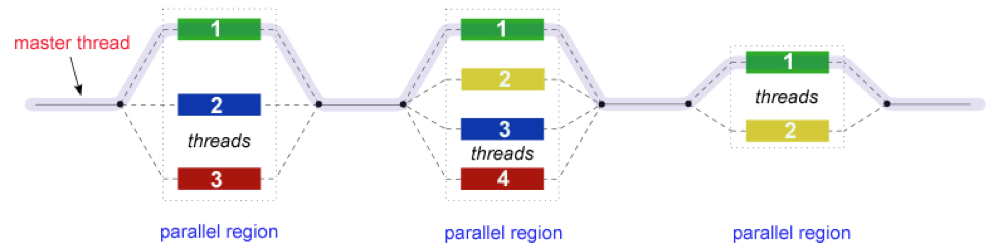
\includegraphics[width=0.60\textwidth]{2_fork_join}
    \bicaption{fork/join模型。}{fork/join model.}
    \label{fig:2_fork_join}
\end{figure}

在POSIX标准中,动态分配的堆内存和全局变量被所有线程共享,这会使多线程编程变得复杂起来。当多个线程要同时访问共享数据时,开发人员必须注意竞争条件和死锁。为了保护临界区,Pthreads提供了互斥量和信号量\citep{grama2003introduction},互斥量可以保证同一时刻至多有一个线程进入临界区,而信号量则允许同一时刻至多有m(m>1)个线程进入临界区。

总体来说,Pthreads并不适合作为通用并行编程的开发工具。虽然它在某些情况下有优势,但是从专业的开发人员的角度看,Pthreads的各组件之间关系复杂,给程序的正确性和可维护性带来了挑战。除此之外,用Pthreads开发的程序不容易扩展到具有大量处理器的环境下\citep{dongarra2003sourcebook},因为在Pthreads中开启线程的数量与可用处理器的个数无关。综上所述,需要开发人员显示管理的线程模型不适合高性能应用的开发。

\subsection{OpenMP}

OpenMP\citep{OpenMP}也是多线程模型,但是OpenMP所支持的共享内存并行编程模型是面向任务的,是对线程更高一层的抽象。

OpenMP提供一套多线程编程API来简化共享内存并行编程,尤其针对高性能应用,它支持大多数共享内存架构。Pthreads仅以库的形式实现,OpenMP的实现则结合了编译制导语句、用于线程管理的运行时环境以及一套库。制导语句指示编译器创建线程、进行同步操作、管理共享内存。因此,OpenMP需要特定的编译器来理解并执行这些制导语句。现在越来越多的编译器开始支持Fortran、C和C++版本的OpenMP。

因为OpenMP专门为高性能应用设计,所以在OpenMP中对线程的使用具有高度的条理性。尤其是按照fork/join模型将串行代码转换为并行代码的过程,一个fork/join块对应于一个并行块(parallel region),并行块用parallel和end parallel制导语句定义。 并行块将一个任务复制到一组线程上运行。然而在并行编程的实践中常见的场景是将多个不同的任务分发到不同的线程上执行,比如并行化的循环。所以OpenMP提供了一些制导原语,使不同任务在不同线程上执行。这个过程叫任务分发(worksharing)。因此,OpenMP最适合并行具有循环体结构的程序\citep{mattson2004patterns}。

OpenMP还提供面向应用的同步原语,进一步简化了并行程序的开发。使用这些原语可以开发出高效的代码,这比配合使用Pthreads的互斥量和条件变量要容易的多。

OpenMP 3.0 在2008年发布\citep{openmp2008spec3},它的一项重要改进就是支持显示的任务(tasks)。这个特性很有用,针对动态产生的任务单元简化了应用程序的并行化,比如递归结构和while循环,这样OpenMP就能够处理图算法和动态数据结构之类的问题了。

OpenMP的特性支持高层次的抽象,非常适合在共享内存系统下开发高性能应用。pragma制导语简化了串行代码转换为并行代码的过程,还有一些制导语简化了并行化循环代码块的过程。在过去,传统的多核机器比较昂贵,OpenMP不能被广泛使用,但是随着近年来多核处理器的普及,OpenMP这种并行编程模型受到越来越多的关注。

\subsection{MPI}

MPI(Message Passing Interface)是一种并行编程模型,进程间的通信是通过互相交换消息完成的。由于不能通过共享变量来实现通信,所以消息传递是分布式内存系统中常用的模型。MPI是目前消息传递模型中主导的标准。
  
MPI\citep{pacheco1997parallel}是对消息传递操作的一系列规定,它是一个库,不是一种编程语言。MPI指定Fortran、C/C++程序中子程序或函数的名字、调用顺序和结果,编译程序的时候要链接MPI库。MPI目前已经是分布式架构下高性能应用开发的事实上的标准,它原生的支持SPMD\citep{mattson2004patterns}(某种程度上是Master/Worker编程模式)。  

MPI实现了消息传递模型\citep{gropp1999using},在改模型下,不同的进程并行执行,每个进程都拥有独立的地址空间。将某个进程地址空间的数据复制到另一个进程的地址空间需要进行通信,这是一种协同操作,第一个进程执行发送(send)操作,第二个进程执行接收(receive)操作。在MPI中,任务划分和分发必须由开发人员实现,这一点跟Pthreads相似,每个进程执行什么任务需要开发人员来显示指定。  

MPI中的通信模式包括点对点通信、集合通信、单向通信和并行I/O操作。点对点通信,比如MPI\_Send/MPI\_Recv,用于两个进程之间的通信。集合通信,比如MPI\_Bcast,用于涉及两个上进程的通信。常规的send/receive操作采用双向模式,发送者和接收者要求能够执行匹配操作。需要一种同步机制来匹配发送操作和接收操作,同时管理存储消息的缓存空间。从MPI-2\citep{mpi2003mpi2}开始支持单向通信,这种通信不再要求发送者和接受者之间的匹配,从而将同步操作和数据传输分离开。单向通信支持远程内存访问(removte memory access),主要提供三个接口:MPI\_Put(远程写),MPI\_Get(远程读),MPI\_Accumulate(远程更新)。并行I/O是MPI-2的重要组成部分,它支持从外部设备获取数据类型和通信子\citep{gropp1999using}。  

另一方面,随着对称多处理(SMP)计算机和多核处理器的普及,消息传递和多线程相结合的编程模型也出现了。在这种混合编程模型下,用户程序由分布在SMP节点或多核处理器上的一个或多个MPI进程组成,每个MPI进程包括多个线程。MPI-2中已经明确定义了MPI程序中MPI和用户创建的线程如何交互,目的是方便用户编写多线程的MPI程序。  

MPI比较适合对可移植性要求比较高的应用,尤其是跨不同的系统和不同时代的计算机,同时也适合使用动态数据结构的应用的任务并行。在过去的20年里(计算机集群时代),消息传递模型,尤其是MPI,已经成为高性能领域的标准解决方案。因此目前大多数科学计算相关的代码都支持在消息传递模型下的并行执行,在某些科学领域,高性能计算指的就是MPI编程。


\subsection{MPI和OpenMP混合并行编程}

将共享内存和分布式内存编程模型结合起来是已经不是什么新想法了\citep{sterling1995enabling},这样做的目标是利用这两种模型的优点:共享内存模型的效率、内存节省和易编程性,以及分布式内存的可扩展性。事实上,这是PGAS模型的最终目标。然而,开发人员不能自己开发新的运行时或语言,但是可以混合已有的编程模型和工具。这种方法称为混合(并行)编程。这种编程模型是当前混合硬件架构的一种现代软件趋势。基本思想是在分布式节点之间使用消息传递(通常是MPI),在单个节点内使用共享内存(通常是OpenMP,甚至是Pthreads)。混合编程还可以使用GPU作为计算能资源。通常使用CUDA,OpenCL也可以使用,但是由于OpenCL直接支持多GPU和GPU + CPU编程,它的使用并没有特别扩展到混合编程领域。

混合MPI/OpenMP编程的基本原理是利用两种编程模型的优势。它将MPI的显式分解和任务放置与OpenMP的简单和细粒度并行化结合起来。因为MPI和OpenMP是行业标准,而且这种模型具有良好的可移植性,这种混合编程模型在SMP集群上被广泛应用。然而,目前还不清楚这种编程模型是否永远是最有效的机制。 实际上,在采用混合编程模型实现之前,必须认真研究代码本身的特性。研究这种混合模型已经有相当多的研究工作了\citep{smith2001development, rabenseifner2003hybrid, estrade2009hybrid}。下面收集了一些组合MPI和OpenMP的合理理由:

\begin{enumerate}
	\item 这种编程模型适合当前的硬件趋势(多核和多处理器)。
	\item 一些应用程序明细有两个级别的并行:粗粒度(适合MPI)和细粒度(最适合OpenMP)。
	\item 在某些情况下,应用程序或系统可能会限制MPI进程(可扩展性问题)的数量,此时OpenMP可以提供额外的并行性。
	\item 有些应用程序在MPI级别上表现出不平衡的工作负载。OpenMP可以通过为每个MPI进程分配不同数量的线程来解决这个问题。
	\item OpenMP避免了MPI引发的计算机节点间额外的通信开销。因此,节点内的内存延迟和数据移动减少了,因为可以在内存上同步,而不是使用同步障碍。
\end{enumerate}

然而,也有一些因素使这种编程模型的效率降低:

\begin{enumerate}
	\item 将OpenMP引入现有的MPI代码意味着引入OpenMP的缺点,例如:
		\begin{enumerate}
			\item 控制任务分配和同步的限制。
			\item 由线程创建和同步引入的开销。
			\item 依赖于编译器的质量和OpenMP的运行时支持。
		\end{enumerate}
	\item 共享内存问题(例如在ccNUMA体系结构中)。
	\item MPI和OpenMP运行时库的交互可能会对程序的性能产生负面影响。
	\item 一些应用程序只具有一层的并行性,引入分层并行模式时可能没有任何好处。
\end{enumerate}

大多数混合MPI/OpenMP的代码都基于层次模型,这使得在MPI层次上发掘大中型粒度的并行性和在OpenMP层次上发掘细粒度并行性成为可能。因此,在高层次上,程序被明确地构造为几个MPI任务,它的顺序代码包含OpenMP指令,以增加多线程特性、利用共享内存。这种编程模型可以以不同的方式实现,这取决于通信和计算的重叠\citep{rabenseifner2003hybrid}。有两个主要类别:没有重叠的通信/计算和有重叠的通信/计算。
  
第一类别不存在MPI调用与其他线程中的其他应用程序代码重叠。这一类别可以以两种方式实现\citep{rabenseifner2003hybrid}:  

\begin{enumerate}
	\item MPI只在并行区域之外被主线程调用。这种方法的优点是在SMP节点内部没有消息传递。因此不需要关心任务的拓扑,因为主线程控制节点之间的通信。缺点是效率可能降低,因为所有其他线程都在主线程通信的时候休眠。此外,MPI库至少必须支持MPI\_THREAD\_FUNNELED级别的线程安全。
	\item MPI在应用程序代码的并行区域之外调用,但是MPI通信是由多个CPU完成的。MPI通信的线程并行化可以通过MPI库自动完成,或者通过应用程序显式地使用完全线程安全的MPI库。
\end{enumerate}

在第一个类别中,非通信线程正在休眠(如果使用非专用节点,则执行另一个应用程序)。下一种MPI/OpenMP方法中解决了CPU空闲的问题。

第二个类别对应于存在重叠的通信和计算。在这里,当通信由主线程(或一些线程)完成时,所有其他的非通信线程都在执行应用程序代码。与前一种情况一样,有两种方法:

\begin{enumerate}
	\item 只有主线程调用MPI例程,即所有通信都汇集到主线程。
	\item 每个线程处理它自己的通信需求,或者通信被汇集到不止一个线程。
\end{enumerate}

第二个类别的主要问题是,应用程序必须被分割两部分代码:一部分代码可以在不访问非本地数据的情况下运行;而另一部分代码需要访问非本地数据,通常会非常复杂。此外,使用这种方法会失去OpenMP的明显优势,因为通信/计算是通过线程的rank(OpenMP的线程ID)来完成的。因此,我们不能使用工作共享(worksharing)指令。最后,线程的通信负载本质上是不平衡的。为了解决这最后一个问题,我们可以使用固定保留或自适应平衡等负载均衡策略\citep{rabenseifner2003hybrid}。  

一旦确定了开发混合应用程序的不同策略,理想的情况是使用以前的方法之一从头开始构建它。但是这并不总是可行的。有时需要从以前的MPI或OpenMP代码构建应用程序。在从初始到混合代码的“改造”过程中,可以考虑到一些问题\citep{estrade2009hybrid}: 
 
 \begin{itemize}
 	\item 用OpenMP改进MPI应用程序。这是最容易的“改造”方法,因为程序状态同步已经被显式地处理了。改造后的优化效果取决于可以使用OpenMP并行化的计算量(通常是循环并行化)有多少。此外,这种“改进”对于通信绑定的应用程序是有益的,因为它减少了需要进行通信的MPI进程的数量。然而,在“改造”过程中,每个节点上的CPU的使用成为一个问题。
 	\item 用MPI改进OpenMP应用程序。这个要复杂一些,因为程序状态必须显式地用MPI处理,需要仔细考虑每个进程如何与其他进程通信。甚至有时可能需要对并行进行完全的重新设计。但是一个成功的“改进”通常会在性能和可扩展性方面带来更大的改善。
 \end{itemize}
 
MPI+ OpenMP方法的一个优点是,MPI单边通信将数据传输与同步分离,而多线程方便了SPMD设计模式的应用。这种混合编程模型在许多应用程序上的应用都获得了明显的性能改进。例如,Bova等已经开发了5个混合编程模型版本的代码\citep{bova1999combining}:CGWAVE,GAMESS,线性代数应用,TLNS3D,以及SPECseis96。布什等\citep{bush2000mixed}已经开发了混合MPI/OpenMP版本的一些内核算法和更大的应用程序。还有一些成功的应用实例:沿海波浪分析\citep{luong2001coastal},大气建模\citep{loft2001terascale},有限元方法的迭代求解\citep{nakajima2005parallel},以及在HeSSE环境下的N-body问题的MPI/OpenMP代码的性能模拟\citep{aversa2005performance}。  
然而这个模型并不总是最有效的可选方法。例如,Cappello和Etiemble\citep{cappello2000mpi},Duthie等\citep{duthie2004mixed},Smith\citep{smith2000mixed},Henty\citep{henty2000performance},Chow和Hysom\citep{chow2001assessing}都在几个例子中表明,不管底层架构如何,纯MPI代码的表现要优于混合的MPI。

\section{PGAS编程模型的相关工作}

\subsection{PGAS编程模型}

分布式共享内存(DSM)模型试图结合共享内存和分布式内存的优点,支持分布式架构中共享内存的概念\citep{protic1995survey}。在DSM模型中,每个处理器按照程序指定的顺序看到自己的内存操作,但是不能保证处理器按顺序查看彼此的操作(和数据)。这导致了内存一致性问题,这是早期DSM系统开发中的一个关键问题。除了内存一致性问题,局部性感知的缺失也是一个重要问题。

PGAS模型是一种实现了局部性感知范式(locality-aware paradigm)\citep{coarfa2005evaluation}的DSM方法。PGAS提供了一个全局地址空间,以及一个显式的SPMD控制模型。PGAS实现通常区分本地和远程内存引用。这样可以利用数据局部性,从而提高分布式内存硬件的性能\citep{saraswat2010asynchronous}。在PGAS模型中,SPMD线程(或进程)共享其部分地址空间的。此外,部分共享空间对于每个线程或进程都是本地的。数据结构可以全局分配,也可以私有分配。全局数据结构在程序员的控制之下分布在不同的地址空间中。任何线程都可以使用远程全局数据进行简单的赋值或解引用操作。编译器和运行时环境负责将这些操作转换为分布式内存机器上的进程之间的消息。因此,使用PGAS模型的程序可以通过使每个线程或进程主要工作在本地来利用局部性。 
 
虽然程序可能只需要通过全局数据结构进行通信,但大多数的PGAS语言都提供了用于批量通信和同步的API。从这个意义上讲,一些库被用作PGAS运行时库。除了运行时库之外,还有专门设计来支持PGAS模型的语言。

\subsection{PGAS运行时库}

PGAS运行时库主要的作用就是将复杂的底层通信进行封装,提供更高层的通信操作的API,同时具有较高的性能。下面介绍三种比较常用的PGAS运行时库:

\begin{enumerate}
	\item GASNet(Global-Address Space Networking )是一个独立于语言的底层网络层,它提供了独立于网络的原语和高性能的单边通信\citep{gasnet}。GASNet旨在作为编译目标和作为运行时库开发的工具。它的设计被分为两层,以最大限度地提高可移植性,同时又不牺牲性能。底层是一个通用接口——GASNet core API,这是基于活动消息(Active Messages)\citep{mainwaring1995active}的,并直接在每个单独的网络架构之上实现的;上一层是一个更丰富、更有表现力的接口,称为GASNet extended API,它提供远程内存访问和各种集合操作等高级操作。在PGAS语言中,Unified Parallel C(UPC)、Coarray Fortran(CAF)、Titanium和Chapel都使用GASNet。
	\item ARMCI(Aggregate Remote Memory Copy Interface)是一个提供远程内存复制功能的库,还包括一组原子和互斥操作\citep{nieplocha1999armci}。ARMCI的开发是由在常规或不规则分布的数据结构、通信库和编译器的环境中支持全球地址空间通信模型的需求驱动的。ARMCI允许单向的put / get操作。ARMCI提供与消息传递库(主要是MPI)的兼容,这对于经常使用混合共享内存编程模型的应用程序是必需的。阻塞和非阻塞API都是必需的,一些应用程序可以使用非阻塞API来重叠计算和通信。
	\item KeLP(Kernel Lattice Parallelism)是一个基于标准消息传递接口MPI的c++类库\citep{kelp}。因此,它充当应用程序和底层通信之间的中间件。KeLP与MPI之间的交互可以简化底层的性能调优。KeLP支持一小部分几何编程抽象来表示数据结构和数据流动。KeLP的数据编排模型将通信模式的描述与这些模式的解释分离开来。程序员使用直观的几何结构来表示数组的动态集合之间的依赖模式\citep{fink1998efficient}。
\end{enumerate}

\subsection{PGAS编程语言}

下面介绍几种实现了PGAS编程模型的编程语言:

\begin{enumerate}
	\item UPC是面向大型并行计算机的高性能计算的C编程语言的扩展\citep{upc}。主要目标是提供对底层机器的有效访问,并为C语言中的并行编程建立通用的语法和语义。UPC结合了共享内存模型的可编程优势,以及对数据布局和消息传递性能的控制。呈现给程序员的是单个共享的分区地址空间,其中的变量可以由任何处理器直接读取和写入,但是每个变量都与单个处理器相关联。UPC使用了SPMD计算模式。在程序启动时,并行性的数量是固定的,通常每个处理器只有一个执行线程。
	\item CAF是Fortran 95的一个小扩展,用于并行处理,现在coarray已经成为Fortran语言定义的一部分\citep{numrich2005co}。coarray扩展解决了任何并行编程模型的两个基本问题:任务分配和数据分布。在任务分配方面,coarray扩展采用了SPMD编程模式。因此,一个程序被复制一个固定的次数。每个复制(称为image)都有它自己的一组数据对象。image的数目可能等于或大于或小于物理处理器的数目,image以异步方式执行。程序员可以通过特定的语句请求同步。另一方面,对于数据分布,coarray允许程序员指定内存映像之间的关系。这很简单,因为coarray就像普通的数组变量,方括号中有一个用于访问image的索引,没有方括号的引用就与本地数据相对应,而方括号引用则涉及图像之间的通信。
	\item Titanium是一种用于高性能并行科学计算的语言和系统\citep{titanium}。Titanium基于java语言,但它并不是一个严格的java的扩展。Titanium对Java的主要扩展是不可变的类、多维数组、一个具有全局地址空间的显式并行的SPMD模式,以及基于区域的内存管理。一个重要的特性是,Titanium程序不需要任何修改就可以分别在单处理器、共享内存机器和分布式内存机器上运行。尽管如此,可能需要进行性能调优来向分布式内存分发应用程序的数据结构。开发团队正在研究程序分析技术的设计和Titanium程序的优化,并考虑开发使用这些技术的编译器和运行时系统。编译器优化代码并将Titanium程序转换成C程序,然后由C编译器编译成本地二进制文件,并连接到Titanium运行时库。
	\item Chapel是由Cray开发的一种并行编程语言\citep{chapel}。Chapel是一种可移植的语言,旨在提高大规模并行计算机的可编程性,赶上或超过MPI等当前编程模型的性能和可移植性。Chapel通过高级抽象的数据并行、任务并行性、并发性和嵌套并行性来支持多线程执行模型。Chapel还包括局部性优化,它提供了对共享数据结构的分配,而不需要对控制结构进行分段。它还通过面向对象的设计和通用编程的特性支持代码重用和快速原型设计。
\end{enumerate}

\section{数据流计算模型}

数据流计算模型是一种数据驱动的并行程序执行模型。数据流程序逻辑基于数据流图表达,是一种优美、直观和强大的并行计算模型,程序单元的输入数据可用时,该程序单元就被激活,当所需资源也可用时就可以在运行时(Runtime)中被执行。数据流是对传统冯诺依曼模型的颠覆式创新,最初由麻省理工学院的Jack B. Dennis教授和他的学生们在上世纪60年代末70年代初提出\citep{dennis1974data},至今40多年的时间中,数据流研究经历了几起几落。随着CPU多核技术的发展,并行对于大规模处理越来越重要;而内存和SSD等存储技术的发展,也使得大数据系统的性能瓶颈逐渐从I/O转向计算。在硬件技术发展与大数据处理需求的双重作用下,数据流以其对并行算法支持的弹性好、扩展性强及性能功耗比高等特点,重新得到学术界和工业界的关注。

数据流模型适用于单机多核环境和分布式集群环境,任务之间的依赖关系可以用有向无环图(DAG)来表示。如图2.2所示,图中的每个节点代表一个任务,具体的任务可以是单机上的一个进程或线程执行的一系列操作,也可以是集群中的一个计算节点对一系列任务的执行;箭头代表任务之间的通信,一个任务完成后,将输出传递给依赖它的任务集,等待输入的任务接收到所有依赖的输入后才开始执行。

\begin{figure}[!htbp]
    \centering
    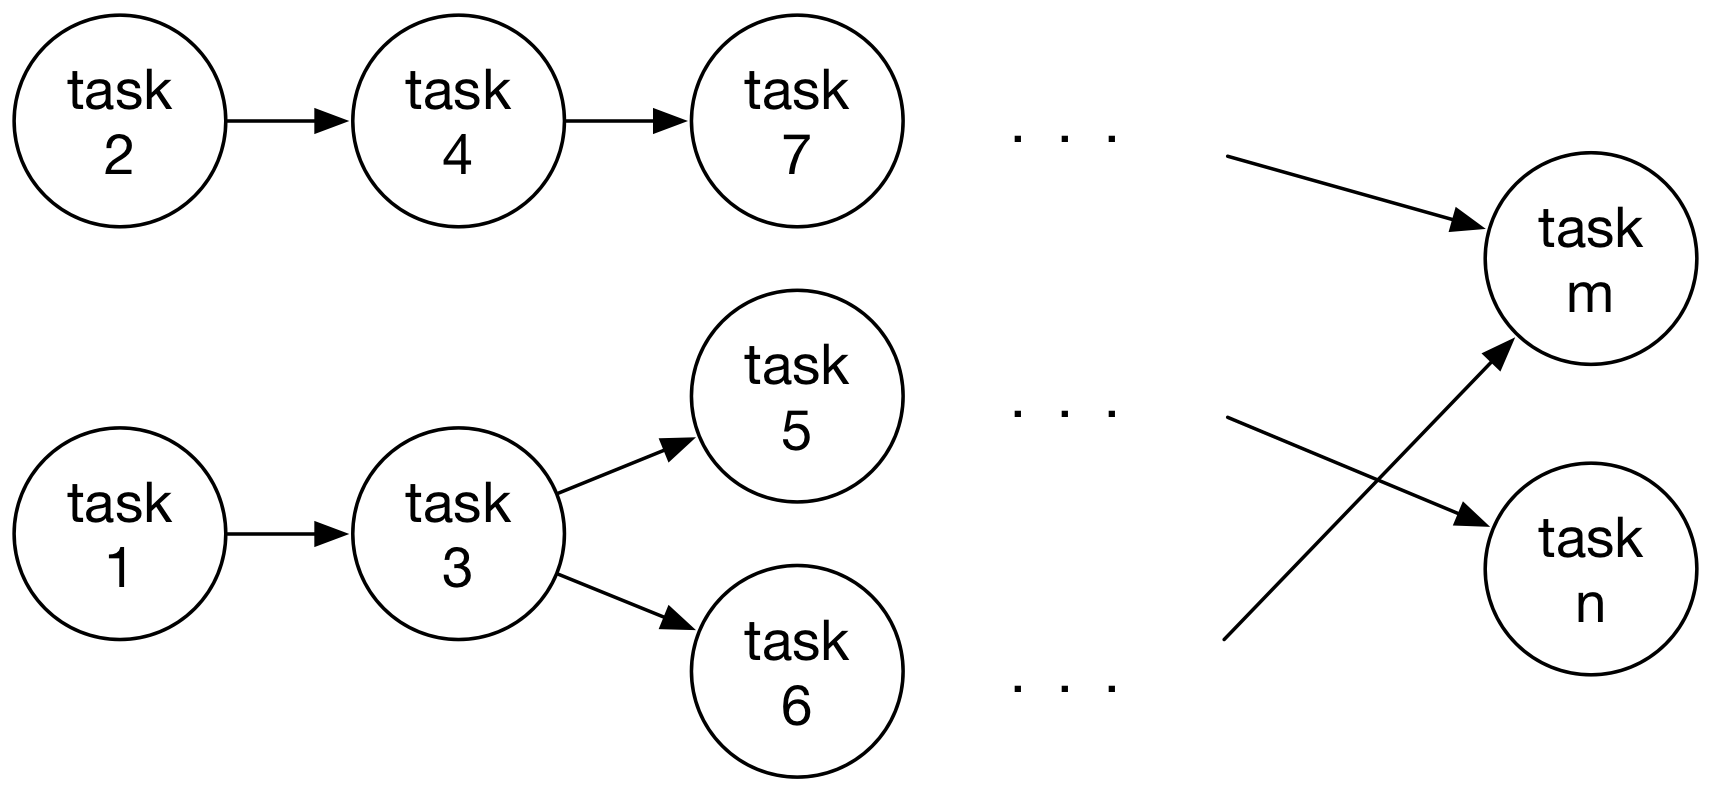
\includegraphics[width=0.40\textwidth]{2_dataflow_dag}
    \bicaption{数据流计算模型DAG示例。}{An example of DAG in dataflow computational model.}
    \label{fig:2_dataflow_dag}
\end{figure}

在大数据和大规模高性能计算的应用需求下,大数据与高性能计算逐渐成为共生关系,对体系结构提出了更高的要求,当前的并行优化技术局限于静态优化,无法满足动态调度、自适应管理和自感知弹性控制的需求。传统OS的垄断地位正在受到挑战,运行时系统软件独技术和学科正在兴起。新的模型和结构需要满足来自五个特性的挑战:

\begin{enumerate}
	\item 可扩展性。体系结构和系统软件的结合和交叉前进,使应用能很好的扩展到超大规模并行平台。
	\item 可编程性。动态细粒度编程模型,显著减少那些影响编程效率的障碍。
	\item 兼容性。去除或显著减少移植到未来平台的约束要求。
	\item 弹性。对软件栈的全部组件提供良好的管理、故障检测和恢复。
	\item 能效。最大化利用动态节能机会,平衡能效、弹性和性能。数据流在上述方面都有其独特的优势,亟待深入研究。
\end{enumerate}

下面介绍三种支持数据流计算模型的架构:Storm、Samza和StarPU。其中,Storm和Samza是工业界认可的实时处理系统,StarPU在科学计算领域有一定的影响力。

\subsection{Storm}

Apache Storm\citep{storm}最开始是由Nathan Marz和他的团队于2010年在数据分析公司BackType开发的,后来BackType公司被Twitter收购,接着Twitter开源Storm并在2014年成为Apache顶级项目。毋庸置疑,Storm已经成为大规模流数据处理的先锋,并逐渐成为工业标准。许多互联网公司都使用Storm来构建实时处理系统,例如国外的Yahoo、Twitter,国内的百度、阿里巴巴。阿里巴巴还基于Storm开发出了更稳定、更快的JStorm\citep{jstorm}。

Storm是原生的流处理系统,提供low-level的API。Storm使用Thrift来定义topology和支持多语言协议,使得我们可以使用大部分编程语言开发,Scala自然包括在内。

\begin{figure}[!htbp]
    \centering
    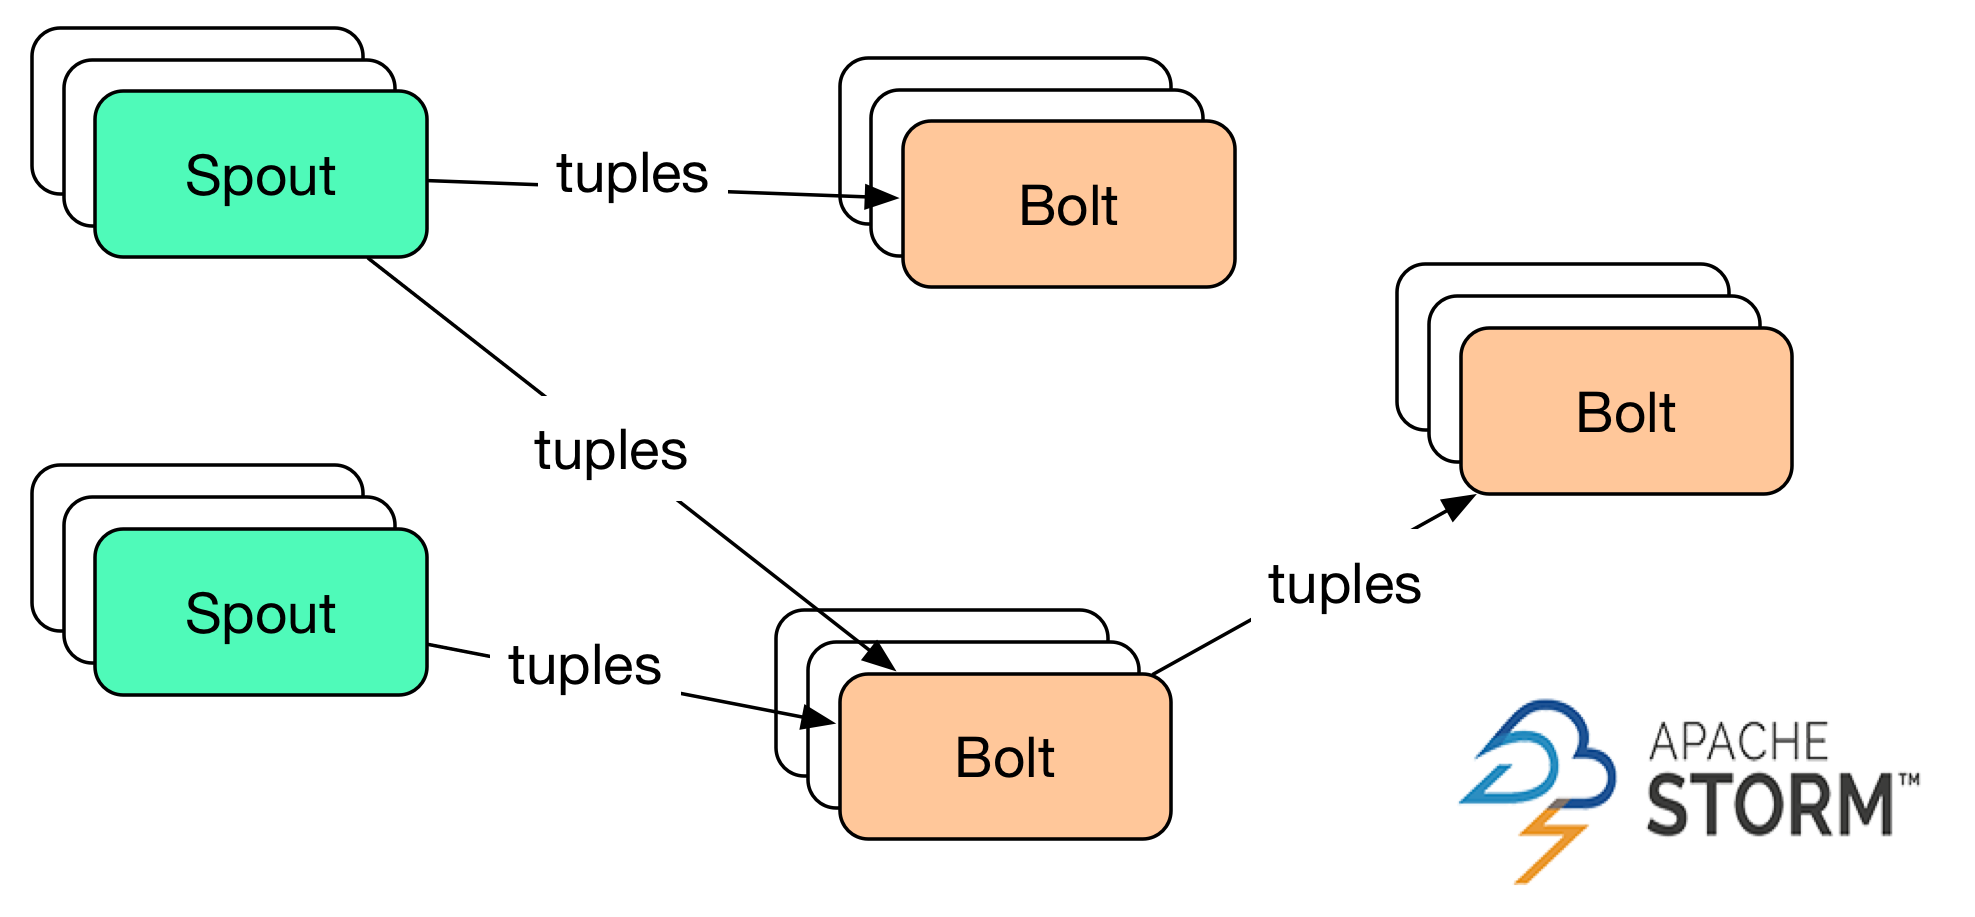
\includegraphics[width=0.40\textwidth]{2_storm_topo}
    \bicaption{Storm中的topology。}{Topology in Storm.}
    \label{fig:2_storm_topo}
\end{figure}

如图2.3,在Storm中,先要设计一个用于实时计算的图状结构,我们称之为拓扑(topology)。这个拓扑将会被提交给集群,由集群中的主控节点(master node)分发代码,将任务分配给工作节点(worker node)执行。一个拓扑中包括spout和bolt两种角色,其中spout发送消息,负责将数据流以tuple元组的形式发送出去;而bolt则负责转换这些数据流,在bolt中可以完成计算、过滤等操作,bolt自身也可以随机将数据发送给其他bolt。由spout发射出的tuple是不可变数组,对应着固定的键值对。

\subsection{Samza}

Apache Samza\citep{samza}是一个开源、分布式的流处理框架,它使用开源分布式消息处理系统Apache Kafka来实现消息服务,并使用资源管理器Apache Hadoop YARN实现容错处理、处理器隔离、安全性和资源管理。Samza在工业界的应用也比较多,像LinkedIn、Uber等公司都有使用Samza来实现各种实时服务。

\begin{figure}[!htbp]
    \centering
    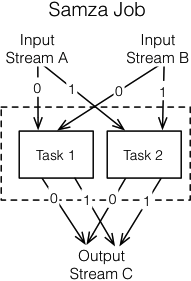
\includegraphics[width=0.30\textwidth]{2_samza_job}
    \bicaption{Samza中的Job。}{Job in Samza.}
    \label{fig:2_samza_job}
\end{figure}

如图2.4,Samza的一个job的基本处理流程是一个用户任务从一个或多个输入流中读取数据,再输出到一个或多个输出流中,具体映射到kafka上就是从一个或多个topic读入数据,再写出到另一个或多个topic中去。多个job串联起来就完成了流式的数据处理流程,Samza中典型的数据流执行图如图2.5所示。

\begin{figure}[!htbp]
    \centering
    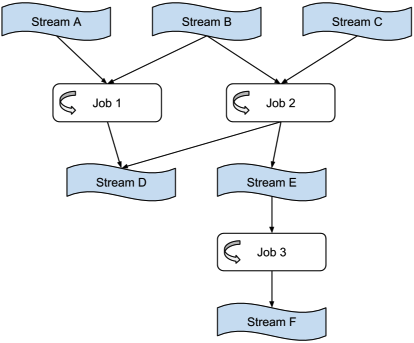
\includegraphics[width=0.40\textwidth]{2_samza_dag}
    \bicaption{Samza中的数据流图。}{Dataflow graph in Samza.}
    \label{fig:2_samza_dag}
\end{figure}

这种模式其实有点像MapReduce的过程,stream输入部分由kafka的partition决定了分区和task数目,类似于一个Map过程,输出时由用户task指定topic和分区(或者框架自动由Key决定分区),这相当于一次shuffle的过程,下一个job读取新的stream时,可以认为是一个reduce,也可以认为是下一个map过程的开始。
不同之处在于job之间的串联无需等待上一个job的结束,类实时的消息分发机制决定了整个串联的job是连续不间断的,亦即流式的。

\subsection{StarPU}

StarPU\citep{augonnet2011starpu}是一个运行时系统,它支持异构多核架构,提供了CPU和加速器的统一视图,将任务高效的映射到异构部件,隐藏了底层细节(如数据传输),充分挖掘CPU和GPU的计算潜力,不必花费大量精力频繁的调整程序来适应不同的目标机器。这样开发人员就不用关心复杂的底层细节问题,可以将主要精力放在算法本身。

StarPU是一个基于任务调度的模型。应用程序提交计算任务,StarPU在CPU和GPU之间对任务和相关的数据传输进行调度,单个任务操作的数据在加速器和主存之间自动传输,开发人员不需要考虑数据传输的问题。StarPU提供高效的任务调度策略:当有任务ready时,调度器将任务插入任务池;worker从调度器获取任务并执行。如果精通调度策略,还可以实现自定义的调度策略。

虽然StarPU的设计偏向于对异构体系结构的支持和优化,但是它的许多设计思想是值得借鉴的,尤其是在调度策略方面。



